\documentclass[10pt,journal,compsoc]{IEEEtran}

\ifCLASSOPTIONcompsoc
  \usepackage[nocompress]{cite}
\else
  \usepackage{cite}
\fi

\ifCLASSINFOpdf
  \usepackage[pdftex]{graphicx}
  \graphicspath{{./images/}}
  \DeclareGraphicsExtensions{.pdf,.jpeg,.png}
\else
  \usepackage[dvips]{graphicx}
  \graphicspath{{./images/}}
  \DeclareGraphicsExtensions{.eps}
\fi

\usepackage{amsmath}
\interdisplaylinepenalty=2500

\usepackage{url}

\hyphenation{op-tical net-works semi-conduc-tor}


\begin{document}

\title{Authentication in the Internet of Things}

\author{Di~Weng,~\IEEEmembership{11621046}
        and~Qi~Song,~\IEEEmembership{21521081}% <-this % stops a space
% \IEEEcompsocitemizethanks{\IEEEcompsocthanksitem M. Shell was with the Department
% of Electrical and Computer Engineering, Georgia Institute of Technology, Atlanta,
% GA, 30332.\protect\\
% % note need leading \protect in front of \\ to get a newline within \thanks as
% % \\ is fragile and will error, could use \hfil\break instead.
% E-mail: see http://www.michaelshell.org/contact.html
% \IEEEcompsocthanksitem J. Doe and J. Doe are with Anonymous University.}% <-this % stops an unwanted space
\thanks{Manuscript received June 28, 2017; revised June 28, 2017.}}

\markboth{Advanced Computer Network, Summer 2017}%
{Di~Weng \and Qi~Song: Authentication in the Internet of Things}


\IEEEtitleabstractindextext{%
\begin{abstract}
The abstract goes here.
\end{abstract}

% Note that keywords are not normally used for peerreview papers.
\begin{IEEEkeywords}
internet of things, authentication.
\end{IEEEkeywords}}


% make the title area
\maketitle

\IEEEdisplaynontitleabstractindextext

\IEEEpeerreviewmaketitle

\IEEEraisesectionheading{\section{Introduction}\label{sec:introduction}}

\IEEEPARstart{T}{he} Internet of Things (IoT) and its related technologies have been actively studied and popularized in the past few years~\cite{DBLP:journals/jnca/AlabaOHA17}. The idea of IoT was originally formulated from the emerging advanced network infrastructures that support a large number of interconnected things or objects, such as Radio-Frequency IDentification (RFID) tags, sensors, personal accessories like smart watches and mobile phones. The objects are then given unique addresses, through which they can communicate and cooperate with each other to complete collective tasks, while the addressing scheme will also enable IoT devices to be identifiable by external services and platforms~\cite{giusto2010internet}\cite{tan2010future}.

However, there is a long-standing argument about the definition of  Internet of Things. IoT is a generic but vague concept with several missing definitions, for example, the range of objects and addressing schemes. This leads to manifold definitions of IoT presented in prior studies. The term, \textit{Internet of Things}, is semantically composed by two words, \textit{Internet} and \textit{Things}, from which two different aspects of IoT technology can be derived, namely, Internet-oriented visions and things-oriented visions, and most of the previous definitions fall into these two categories. Additionally, some other studies suggest that the third aspect, semantic-oriented visions, is also a part of the IoT framework. These three visions (Fig.~\ref{fig:visions}) are discussed as follows:

\begin{figure}[htbp]
	\centering
  	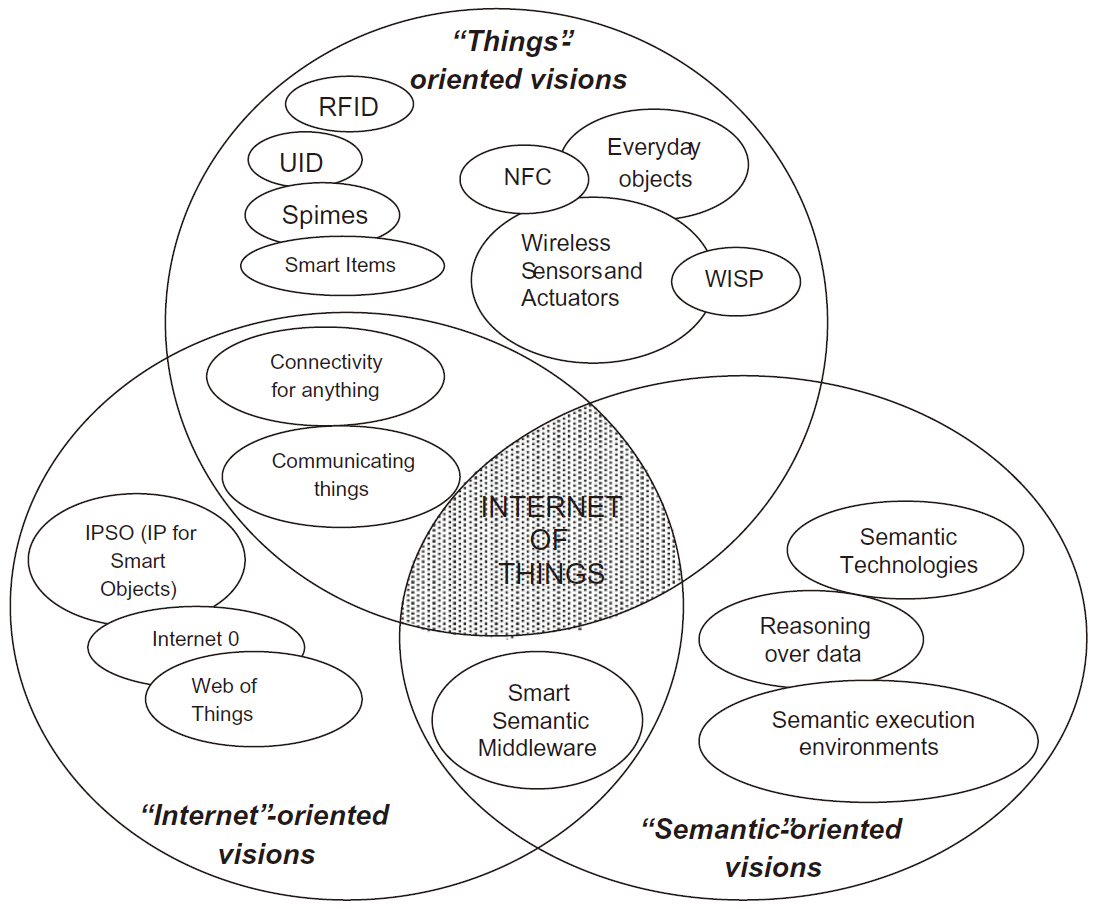
\includegraphics[width=0.45\textwidth]{visions}
  	\caption{Three visions of the Internet of Things paradigm by L. Atzori et al.~\cite{DBLP:journals/jnca/AlabaOHA17}, including Internet-oriented visions, Things-oriented visions, and Semantic-oriented visions. Their relations and components are  described in a Venn diagram.}
  	\label{fig:visions}
\end{figure}

\textbf{Internet-oriented visions} focus on the connectivity of objects inside the IoT framework. Since Internet Protocol (IP) has been widely adopted in traditional network infrastructures and is already connecting millions of devices around the world, most of the definitions in the realm of Internet-oriented vision attempt to reuse lightweight variants of the IP stack to address the connectivity issues among IoT objects. One of the definitions is canonicalized by IPSO (Internet Protocol for Smart Objects) Alliance~\cite{vasseur2008ip}, an international organization consisting of 26 companies, including several notable manufacturers of embedding processing units like ARM and Intel. IPSO Alliance proposes the usage of IP architecture on the basis of communication techniques with low power consumption like IEEE 802.15.4 and 6LoWPAN~\cite{culler20096lowpan}. The integrated IPv6 technology  provides sufficient address space for IoT objects, and low-power design enables resource-constrained IoT devices to communicate at a lower rate but consume less power. There are other similar approaches like Internet {\O}, allowing ``IP over anything'' by reducing the complexity of the IP stack.

\textbf{Things-oriented visions} advocate wide-spread Radio-Frequency IDentification (RFID) tags as \textit{things} in the IoT framework. By attaching RFID tags to everyday objects, Things-oriented visions enable users of IoT to track and identify these objects. The idea was first established by Auto-ID Labs~\cite{Auto-ID_Labs_2017-06-26}, and later generalized by several studies~\cite{epcglobal2004radio}\cite{DBLP:conf/icse/2006}, which further extend identifiable tags into a Unique/Universal/Ubiquitous IDdentifier (UID) architecture. While the definition of IoT presented by these visions narrows it down to mere object identification, the maturity of RFID technologies and the popularity and enthusiasm in the business community show a promising adoption rate of such architecture. Moreover, by combining things-oriented visions with Internet-oriented visions, several unified definitions were proposed regarding both the identification and connectivity of objects, as stated by the European Commission\cite{bassi2008internet}:
``Things having identities and virtual personalities operating
in smart spaces using intelligent interfaces to connect
and communicate within social, environmental, and user
contexts.''

\textbf{Semantic-oriented visions} arise from the literature under an assumption that the number of interconnected objects exhausts the capability of direct management, where the organization of the information generated by these objects becomes challenging. Such issue can be addressed by integrating semantic technologies like data reasoning and semantic execution environment into the IoT framework~\cite{toma2009joint}.

As a promising technology, IoT was included in the list of six ``Disruptive Civil Technologies'' that will potentially generates huge impacts on US national power~\cite{council2008six}. US National Intelligence Council, the author of the list, claimed that
``popular demand combined with technology advances could drive widespread diffusion of an Internet of Things (IoT) that could, like the present Internet, contribute invaluably to economic development.''
Despite IoT's contribution to human's everyday life, it also brings severe security risks along the way due to its wide distribution and applicability. It is also stated in the aforementioned report that
``to the extent that everyday objects become information security risks, the IoT could distribute those risks far more widely than the Internet has to date.''

Four categories of security issues in the IoT framework are summarized by Alaba et al.~\cite{DBLP:journals/jnca/AlabaOHA17}, including application, architecture, communication, and data. With authentication and access control technologies, traditional computer networks have resolved a variety of security and privacy issues in three ways~\cite{DBLP:conf/icdcsw/LiuXC12}: a) forbid unauthorized users to access resources; b) prohibit authorized users from accessing resources beyond their privileges; and c) grant correct resource access to authorized users. As a key issue in both categories of application and architecture, authentication technologies continues playing an important role in the security of IoT.

Two challenges arise while applying existing authentication techniques to the application and architecture of IoT devices. First, most of the IoT devices are resource-constrained, where most of the strong cryptography methods currently used cannot be computed fast enough to match the power supply of devices and the rate of information sensing. Second, the complex environment of IoT networks requires an extensible and scalable authentication scheme. The number of devices in an IoT network could scale up to millions, introducing difficulty in many aspects of traditional authentication, such as the distribution and revoking of symmetric encryption keys.

Apart from the machine authentication of IoT, which mainly consists the authentication of application and architecture as stated above, user authentication~\cite{o2003comparing} is also an essential part of IoT security paradigm. By integrating user authentication, IoT devices like mobile phones are able to identify owners with simple interactions and protect sensitive personal information from unauthorized users.


The work of this survey is divided as follows:

\begin{itemize}
	\item \textbf{Presentation:} Qi Song presented the assigned paper~\cite{DBLP:journals/tifs/FrankBMMS13}, and Di Weng presented the survey on the authentication of the Internet of Things;
	\item \textbf{Writing:} Section \ref{sec:introduction}, \ref{sec:application}, and \ref{sec:conclusion} were written by Di Weng, and Section \ref{sec:architecture} and \ref{sec:user} were written by Qi Song.
\end{itemize}

This survey is organized as follows: the machine authentication of IoT is covered in Section \ref{sec:application} and \ref{sec:architecture}, which explain the authentication in IoT applications and architecture, respectively; then, Section \ref{sec:user} summarizes the user authentication in IoT framework briefly; finally, this survey is concluded in Section \ref{sec:conclusion}.

\section{Application Authentication\label{sec:application}}

Recent years have witnessed the great impacts brought by the Internet of Things technologies via a variety of applications. Applications of IoT can be categorized by: network type, scope, scale, heterogeneity, repeatability, and the involvement of users~\cite{DBLP:journals/fgcs/GubbiBMP13}. However, it remains a crucial challenge to protect the application data authentic and intact with authentication technologies while transmitting the data over IoT networks.

Studies depict that the authentication in IoT applications generally involves two validation aspects corresponding to different concerns~\cite{DBLP:journals/jnca/AlabaOHA17}: a) peer authentication: \textit{how does a IoT device recognize and trust its peers}; and b) data origin authentication: \textit{how to ensure the origin of data is an authentic IoT peer}. These two validation aspects were proposed to enhance the security of machine-to-machine (M2M) communications~\cite{martin2016authentication} in IoT framework based on the complicated environment of IoT networks, which may comprise enormous cheap yet resource-constrained devices in contrast to traditional networks with a few hundred powerful nodes.

Several research attempts were made regarding the authentication of IoT applications. One of the earliest studies in this area was conducted by Liu et al.~\cite{DBLP:conf/icdcsw/LiuXC12}, in which they proposed an authentication and access control scheme based on Elliptic Curve Cryptography (ECC) combining both asymmetric and symmetric encryption methods. Registration Authorities (RA), a type of standalone authorization servers in IoT networks, are established to recognize the authenticity of both devices and users with predistributed certificates signed by the generated elliptic curve. Regular Elliptic Curve Diffie-Hellman (ECDH) key exchanging protocol is then performed between RA and users. This work also takes multiple domain authentication into consideration by adding a Home Registration Authority (HRA) and providing a Single Sign-On (SSO) solution for IoT users. Ndibanje et al.~\cite{DBLP:journals/sensors/NdibanjeLL14} presented a comprehensive analysis of security weaknesses in this method and proposed further improvements concerning the message exchanging performance and security assessment of the protocol.

In addition to ECC, other encryption techniques have been introduced to address the authentication issue in IoT applications as well. Attribute-Based Encryption (ABE) was adapted for the authentication of resource-constrained IoT devices by Yao et al.~\cite{DBLP:journals/fgcs/YaoCT15}. ABE is a cryptography method based on Identity-Based Encryption (IBE) aiming to produce encrypted texts recognizable by users with certain identities only. Extended from IBE, ABE identifies users with a set of predefined attributes. Only users with the specific combinations of attributes corresponding to the defined access policy are allowed to decrypt the cipher text, enabling broadcast encryption of the application data. However, the bilinear Diffie-Hellman scheme used by ABE is slow and computationally-intensive, which is proven unsuitable for IoT devices. Yao et al. replace bilinear Diffie-Hellman scheme of general ABE with faster elliptic curve scheme, leading to better performance and improved bit security. However, the proposed method still exhibits several inherent limitations as discussed in the paper: a) poor flexibility in revoking attributes; b) poor scalability with communication and computational overhead; and c) poor generality with multiple-authority applications.

The perception layer emerges from the evolution of IoT technologies as a substantial number of sensors are being deployed in IoT networks. Despite the significant importance of perception layers, only a few studies focus on the authentication issue of these layers. Ye et al.~\cite{ye2014efficient} presented an efficient authentication and access control scheme between users and the perception layer in Wireless Sensor Networks (WSN) by exploiting ECC key exchanging protocol with a mutual authentication style comprising two phases, namely, authentication and key establishment. A lightweight authentication protocol specifically designed for securing RFID tags was also proposed~\cite{al2016car} in the literature. Nonetheless, such authentication issues, for example, how to segregate and protect sensitive application data in the heterogeneous perception layer of IoT networks, remain largely unsolved.

Neisse et al.~\cite{DBLP:journals/compsec/NeisseSFB15} proposed SecKit, a model-based security toolkit, to address security policy management issues in IoT. By analyzing the characteristics of IoT framework comprehensively, authors designed the toolkit to support various application scenarios: a) dynamic context; b) trust management; c) digital divide; d) data flow control; e) actuator action control; and f) data anonymization. Moreover, authors formalized the security management procedure by identifying several metamodels involved in the process, including data, time, identity, role, context, structure, behavior, risk, trust, and rule. These metamodels were then implemented using the Eclipse Modeling Framework (EMF). Such formalization demonstrates the feasibility of the proposed toolkit and assists the administrators of IoT networks in creating, modifying, and enforcing security policies at a fine-grained level.


\section{Architecture Authentication\label{sec:architecture}}

\section{User Authentication\label{sec:user}}

\section{Conclusion\label{sec:conclusion}}

The conclusion goes here.

\newpage
\bibliographystyle{abbrv}
\bibliography{survey}

\end{document}


